\documentclass[a4paperm]{article}
%\documentclass[12pt,twocolumn]{article}

\usepackage[T2A]{fontenc}
\usepackage[utf8]{inputenc}
\usepackage[russian,english]{babel}
\usepackage{amsmath,amsthm,amssymb,stackrel}
\usepackage[affil-it]{authblk}
\usepackage{cite}
\usepackage{scrextend}
\usepackage{verbatim}
\usepackage{paralist}
\usepackage[mediumspace,mediumqspace,Grey,squaren]{SIunits}
\addtokomafont{labelinglabel}{\sffamily}
\usepackage{amsmath}
\usepackage{graphicx}
 \usepackage[usenames, dvipsnames]{color}
 \usepackage{multirow}
 \usepackage{longtable}
 \usepackage{lineno}
 \usepackage{textcomp}
 
 \usepackage{xr}
 \usepackage{longtable}
 \usepackage{array} 
 \usepackage{inputenc} 
 
%\usepackage[none]{hyphenat} %no nyphenation

\usepackage{SIunits}
\usepackage{miller}
\usepackage[version=3]{mhchem}

\usepackage{float} %H with figures

\setlength{\parindent}{5ex}

 \usepackage{newfloat} %For numbering of supplemmentary figures
 \DeclareFloatingEnvironment[name={Supplementary Figure}]{suppfigure}

\graphicspath{{figures/}}
\externaldocument{SI/smose_supp}

\usepackage[outdir=./]{epstopdf}



\begin{document}

%\linenumbers

\title{Janus structures of SMoSe and SVSe compositions with low enthalpy and unusual crystal chemistry}



\author[1,2,3]{Pavel N. Gavryushkin
   \thanks{Electronic address: \texttt{gavryushkin@igm.nsc.ru, p.gavryushkin@g.nsu.ru}; Corresponding author}}     
\author[2]{Nursultan Sagatov}
\author[1]{Ekaterina V. Sukhanova}
\author[4]{Inna V. Medrish}
\author[1]{Zakhar I. Popov}


\affil[1]{Emanuel Institute of Biochemical Physics of Russian Academy of Sciences, 4 Kosygin Street, Moscow, 119334, Russian Federation}
\affil[2]{Sobolev Institute of Geology and Mineralogy, Siberian Branch of Russian Academy of Sciences, prosp. acad. Koptyuga 3, 630090 Novosibirsk, Russian Federation}
\affil[3]{Novosibirsk State University, Pirogova 2, Novosibirsk 630090, Russian Federation}
\affil[4]{Samara Center for Theoretical Material Science (SCTMS), Samara State Technical University, Molodogvardeyskaya St. 244, Samara, Russia 443100}


\date{}
\maketitle

%\linenumbers

\begin{abstract}
The recent synthesis of single-layer Janus type transition metal dichalcogenides (TMDs) raise the question of the existence of other possible 2D structures with an asymmetric out-of-plane structural configuration.
In the present work, we perform the theoretical search for the new Janus structures having SMoSe and SVSe compositions. We performed the detailed crystal-chemical analysis of the predicted structures and showed that some of the dynamically stable structures are characterized by the unique for TMDs crystal-chemical features, among which are quadruple Mo-Mo bonds and covalent S-S, Se-Se bonds. We also illustrated the tendency of Mo-bearing TMDs to form strong Mo--Mo bonds with chains or isolated dimers of molybdenum atoms while in the case of vanadium-containing TMDs this feature is not characteristic. Two predicted crystal structures, called as 1M-SVSe and 1A'-SMoSe, are especially promising for experimental synthesis and practical application due to their dynamical stability and rather low value of the enthalpy compared to known structures: the enthalpy of the 1M-SVSe is 0.22 ev/f.u. lower than that of 1T-SVSe, while the enthalpy of 1A'-SMoSe is 0.12 ev/f.u. lower than the enthalpy of 1T-SMoSe. The performed topological analysis showed that the predicted structures are unique and do not have analogs in the ICSD database.
\end{abstract}


\begin{comment}
\section*{Phase renaming}
fes = 1S \\
fxt = 1H' \\
T-hor-SVSe = 1M-SVSe \\
H-hor-SMoSe = 1M'-SMoSe \\
SVSe-airss1 = 1A-SVSe \\
SMoSe-airss1 = 1A'-SMoSe \\
SVSe-airss3 = 1A''-SVSe \\
SMoSe-airss3 = 1A'''-SMoSe \\
test1 (SMoSe) = 1O \\
test2 (SMoSe) = 1O' \\
test3 (SMoSe) = 1M'' \\
\end{comment}


%%%%%%%%%%%%%%%%%%%%%%%%%%%%%%%%%%%%%
\section*{Introduction}
%%%%%%%%%%%%%%%%%%%%%%%%%%%%%%%%%%%%%

Transition metal dichalcogenides (TMDs) represent a wide family of materials consisting of transition metal (TM) of group IV--VI surrounded by chalcogen atoms (Ch): S, Se, or Te. 
TMDs crystallize in four main structural types: CdI$_2$, MoS$_2$, FeS$_2$-pyrite, and less frequently -- in FeS$_2$-marcasite structural type \cite{wells}.

The first two structural types are characterized by the layered structures with MX$_2$ sandwiches bonded by the weak Van-der-Waals interactions and, therefore, the crystals can be exfoliated into individual stable layers \cite{zhang2020intercalation}. These quasi-2D sandwiches attract considerable attention due to their wide range of properties \cite{li2017graphene, SHI20181, xi2016ising, hu2019recent, pi2019recent}. 
Particularly, the TMDs can act as semiconductors \cite{nayeri2018transport}, metals \cite{zhao20212d}, semimetals \cite{xu2020high, zhao2020observation}, or superconductors \cite{wang2020nodeless,hsu2017topological} which make the family of TMDs suitable for a lot of applications. 


At ambient conditions the MX$_2$ (M=Mo, W, X=S, Se) compounds crystallize in the archetype molybdenite structure (MoS$_2$) which consists of close-packed layers of chalcogen atoms placed exactly one under/above another and TM atoms occupied one-half of the trigonal prismatic cavities located between the layers of chalcogen atoms. 
In the most stable polytype of molybdenite, X--M--X multiplet layers are arranged similar to the close-packed layers of {\it hcp} structure, i.e. with periodicity through each two layers (Figure \ref{1H1T}a).
Due to hexagonal symmetry, this structure of TMDs can be denoted as 2H according to Ramsdell notation.
In the present work, we do not consider the stacking sequence of X--M--X sandwiches, and the structures will be designated as 1H, 1T, 1H' and etc.


X--M--X sandwich, consisting of three layers, in crystal-chemical community, usuallyь is termed as {\it multiplet layer}, while in the community of low-dimensional material scientist -- as {\it monolayer}.
Here we will follow the last tradition. 


If one layer of chalcogen atoms in the X--M--X monolayer is shifted, the coordination polyhedron of TM atom is changed from a trigonal prism to a octahedron (Figure \ref{1H1T}b). 
The monolayer of such a structure has a trigonal symmetry and can be designated as 1T \cite{huang2020recent}. 
The deformed 1T structure with chains of Mo atoms connected by the shorter bonds is denoted as 1T' \cite{huang2020recent}.
Depending on the exact chemical composition of the TMD monolayer, either trigonal prismatic or octahedral phase are preferable \cite{ataca2012stable}.
For instance, in the case of the molybdenum disulfides, diselenides, and ditellurides the 1T-phase is less energetically favorable than the 1H-phase. However 1T structure can be obtained by means of intercalation \cite{kan2014structures, wang2014atomic}, deformation \cite{duerloo2014structural} or surface functionalization \cite{tang2015stabilization, voiry2015covalent}. 

Recently, compounds of a new subclass of TMDs in which the top and bottom layers are formed by different chalcogen atoms (so called Janus structures) were fabricated and attracted significant interest \cite{lu2017, zhang2017janus} of the researchers. 
The opportunity to change the top layer of atoms opens an additional degree of freedom to manipulate the properties of TMDs. 
Janus structures have structural symmetry breaking \cite{li2017electronic, van2020first} resulting in Rashba spin splitting \cite{hu2018intrinsic} and transverse dipole moment leading to large piezoelectricity \cite{dong2017large, li2018recent}. 
The Janus structures of TMDs have a lot of potential applications, for example in water-splitting \cite{xia2018universality, ma2018janus} or hydrogen evolution reaction \cite{er2018prediction, zhou2019janus}. 
Theoretical investigations showed that, as in the case of pristine monolayers, Janus TMDs with different chemical compositions can be thermodynamically stable in the 1H or 1T structures described above.
Meanwhile, the different chemical composition of the top and bottom layers assumes the possibility for the stabilization of the new structures, substantially different from known 1H, 1T or 1T'.
Based on this assumption we performed the search for the new Janus TMDs structures using unbiased methods of crystal structure prediction, which have not been performed yet.


\begin{figure}
        \includegraphics[width=0.4\textwidth]{1H1T.png}
        \caption{Packing of trigonal prisms and octahedra in 1H (a) and 1T (b) structures of SMoSe.}
\label{1H1T}
\end{figure}





%%%%%%%%%%%%%%%%%%%%%%%%%%%%%%%%%%%%%
		\section{Methods}
%%%%%%%%%%%%%%%%%%%%%%%%%%%%%%%%%%%%%

%%%%%%%%%
\subsection*{Crystal structure prediction}
%%%%%%%%%

The search for the lowest-enthalpy monolayer structures with SMoSe and SVSe compositions was performed using evolutionary algorithms implemented in the USPEX program package \cite{uspex1,uspex2,uspex3} and the random sampling method implemented in the AIRSS software \cite{airss1,airss2}.

The crystal structure search within USPEX was performed in fixed composition mode with 2--6 formula units per unit cell.
The number of structures in the first generation of the calculations was equal to 180.
Half of the structures with the lowest enthalpy were selected after the optimization and then used to produce the next generation.
A new generation was produced as follow: 50\% of all structures were generated by heredity, 10\% -- by atomic mutation, 10\% –- by lattice mutation, and 30\% –- randomly.
On average, 40--47 generations were produced and relaxed.
Using AIRSS program about 5000--6000 structures were randomly generated and optimized for compounds with 4 and 6 formula units per unit cell and structures with the lowest enthalpy were selected. 
In both USPEX and AIRSS calculations, to avoid adjacent layers interactions, a vacuum layer in a direction perpendicular to the plane of the layer ($c$-axis) was set to be more than 15 \AA.
 
The total energies and forces were calculated by solving the Schr\"{o}dinger equation based on projector augmented plane-wave implementation \cite{blochl1994projector} of density functional theory (DFT) using the VASP program package \cite{vasp1,vasp2}.
Exchange correlation effects were treated in the generalized gradient approximation (GGA) with Perdew-B\"{u}rke-Ernzerhof scheme \cite{pbe}.
In case of SVSe structures, Dudarev’s GGA+U method \cite{gga+u} with $U-J$ = 3 eV was used \cite{PhysRevB.93.054429,C6CP06732H}.
Pseudo-potentials with $4p^6 5s^1 4d^5$ (Mo), $3p^6 3d^4 4s^1$ (V), $3s^2 3p^4$ (S), and $4s^2 4p^4$ (Se) electrons were used.

In all crystal structure prediction calculations medium-quality optimization was performed using the conjugate gradient method \cite{conjugate_gradient}. 
The energy cutoff of plane waves was set to 420 eV and 700 eV for the intermediate structures and then for the most promising of them. 
The first Brillouin zone was sampled according to Monkhorst-Pack scheme \cite{monkhorst1976special} with the density of k-points being equal to 0.5 \AA$^{-1}$ and 0.2 \AA$^{-1}$, respectively. 
The manually produced structures were optimized with the same high-quality optimization parameters.

To test the proposed methodology of crystal structure prediction, we revealed not only the well known 1H, 1T, and 1T' structures but also recently suggested 1H' and 1S, using both USPEX and AIRSS. 


To study a dynamic stability of predicted structures phonon dispersion spectra were calculated within the PHONOPY code \cite{phonopy}. 
We used VESTA program for crystal structures visualization \cite{momma2011vesta} and instruments of Bilbao Crystallographic server -- for the structures symmetrization \cite{bilbao}.



%%%%%%%%
\subsection*{The topological search}
%%%%%%%%

Within the topological search, original structural information was selected from the Inorganic Crystal Structure Database (ICSD, release 2020/2) \cite{icsd_1} and Cambridge Structural Database (CSD, release 2021) \cite{icsd_2} 
In this case, the procedures of screening  by the methods of the combined geometric-topological analysis with ToposPro (http: //topospro.com) package have been used \cite{topos_1}. 

We use bold three-letter symbols of the Reticular Chemistry Structure Resource nomenclature (\cite{rcsr}, http: //rcsr.anu.edu.au/) or ToposPro NDk-n symbols \cite{rcsr_2}) to designate the topological types of the underlying nets.
The topology of an underlying net was determined in an automated mode by comparison of a set of topological indices of the net with those for the reference nets from the ToposPro TTD collection \cite{TTD}.

For the topological analysis, we have used only fully solved crystal structures without errors in the determination of interatomic bonds or chemical composition.
The nets of interatomic bonds were determined by the Domains methods using the program AutoCN \cite{blatov2016_rods}. 
Only strong interatomic bonds with solid angles of the faces of Voronoi-Dirihle polyhedron ($\Omega \geq 5 $ of the whole 4$\pi$ solid angle) were considered.
Structures with great values of unit cell parameters were excluded from the consideration.
For instance, we did not consider polytypes of ZnS with cell parameters more than 50 \AA.

Earlier the numerous structural relations between unhydrous simple salts and more simple binary inorganic compounds have been shown \cite{blatov2011_salts, medrish2020_zintl}. 
Due to this well-known structural phenomena, we analyse topology not only for the complete  representation, but also the topology of the underlying net.
In the complete representation, the net corresponds to the all strong interatomic bonds, while the underlying net is determined between metals and centers of ligands.

Due to the short interatomic bonds, the topologies were not determined for the crystal structures 1A, 1A', 1H', and  1M''.


%%%%%%%%%%%%%%%%%%%%%%%%%%%%%%%%%%%%%
			\section{Results}
%%%%%%%%%%%%%%%%%%%%%%%%%%%%%%%%%%%%%

\subsection{Earlier known MX$_2$ structures}

According to the calculations performed, 1H structure is the most energetically favorable in the case of SMoSe composition  (Table \ref{t:enthalpy}) which is consistent with previously reported results \cite{wang20182h}. 
But in the case of SVSe composition, the most energetically favorable structure is 1T' monolayer (Table \ref{t:enthalpy}). 
It is well known that enthalpy difference of V-based dichalcogenide phases is sensitive to computational parameters \cite{C6CP06732H}. 
In the framework GGA+U approach at the U$_eff$>2.5, the 1T phase of VS$_2$ becomes energetically favorable \cite{PhysRevB.93.054429} in contrast to HSE06, which displayed lower energy for the 1H-VS$_2$ configuration.
A small difference in energy between the phases of the V-based dichalcogenides shows the necessity of a careful choice of calculation method for an accurate description of the atomic and electronic structure \cite{C6CP06732H}.

The previously proposed 1S and 1H' structures \cite{tang2021_janus,ma2016_fxt}, also designated as $fxt$ and $fes$ \cite{PhysRevB.93.035442, Terrones_2014,PhysRevB.92.085427},  have close values of enthalpy.
For both SMoSe and SVSe compositions, 1S structure is more energetically favourable than 1H' and the enthalpy difference is equal to 0.01 eV/f.u. for SMoSe and 0.06 eV/f.u. for SVSe (Table \ref{t:enthalpy}).
Also for both SMoSe and SVSe, 1H' and 1S structures are less preferred than 1H, 1T, and 1T' structures (Table \ref{t:enthalpy}).

1H, 1S, and 1H' are characterised by the trigonal prismatic coordination polyhedron, and the difference between these structures is in the manner of interconnection of trigonal prisms. 
In 1S and 1H', trigonal prisms share not only common edges, as in 1H, but also common faces (Figure \ref{fes_fxt}).
Edge-sharing interconnection of trigonal prisms realized in 1H' and 1S structures inevitably results in the appearance of the cavities greater in volume than the cavities of 1H and 1T, which provide the most uniform distribution of the Ch and TM atoms. 
Cavities of 1S have the form of the slightly compressed cube (Figure \ref{fes_fxt}a) and the volume of these cavities is almost two times greater than the volume of the cavities in the 1H structure.
In case of SMoSe, the cavities have the volumes 38.8 \AA$^3$ and 17.7 \AA$^3$, respectively.
The volume of hexagonal cavities of 1H' structure (Figure \ref{fes_fxt}b) is almost eight times greater than the volume of cavities in the 1H phase, 137.8 \AA\ against 17.7 \AA$^3$.




%%%%%%%%%%%%%%%%%%%%%%%%%%%%%%%%%%%%%
		\subsection{New structures}
%%%%%%%%%%%%%%%%%%%%%%%%%%%%%%%%%%%%%

New crystal structures were produced in two different ways, in an automated manner by USPEX or AIRSS, and analytically -- based on the 1H structure.


The new structures are characterized by triclinic, monocliniс, and orthorhombic symmetries and we will designate them as 1A, 1M, and 1O, respectively.
To distinguish structures with the same symmetry we will use single quotes.
For instance, {\it 1A, 1A', 1A''}, and {\it 1A'''} are the crystal structures with triclinic symmetry having sufficiently different atomic arrangements.



%%%%%%%%%%%%%%%%%%%%%%%%
\subsubsection{The structures revealed with {\it unbiased} algorithms}
%%%%%%%%%%%%%%%%%%%%%%%
Table \ref{t:enthalpy} shows the values of the predicted structures, figures \ref{phon_smose} and  \ref{phon_svse} -- their phonon dispersion curves. 

Among the predicted structures, 1M-SVSe and 1A'-SMoSe are the most promising ones, because in addition to dynamic stability the formation enthalpies of 1A'-SMoSe and 1M-SVSe are lower than that of 1T structures with the same compositions.


In the case of SMoSe composition, 1M', 1A''', and 1M'' crystal structures are dynamically stable, but energetically they are less favourable than 1H or 1T (Figure \ref{phon_smose}, Table \ref{t:enthalpy}).
For SVSe composition, 1A and 1A'' structures also show dynamic stability (Figure \ref{phon_svse}). 

To simplify the description of the structural relations between numerous revealed structures, below we showed in pairs crystal structures obtained through the optimisation of the same structure and these structures will be described together.
The dynamically stable structures are highlighted in bold, and only these structures will be considered further.


\begin{tabbing} 
	AAAAAAAAAA \= AAAAAAAAA \kill
	{\bf 1M-SVSe} \> 1M-SMoSe \\
	1M'-SVSe \> {\bf 1M'-SMoSe} \\
	{\bf 1A-SVSe} \> {\bf 1A'-SMoSe} \\
	{\bf 1A''-SVSe} \> {\bf 1A'''-SMoSe} \\
	
	1O-SVSe \> {\bf 1O-SMoSe} \\
	1O'-SVSe \> 1O'-SMoSe \\
	1M''-SVSe \> {\bf 1M''-SMoSe}
\end{tabbing}

\begin{table}[H]
	\caption{Calculated enthalpies of SMoSe and SVSe structures.} \label{t:enthalpy} \vspace{2mm}
	\centering
	\begin{tabular}{l*{5}{l}}
		\hline \hline
		\multirow{2}*{Phase} & \multicolumn{2}{c}{Enthalpy (eV/f.u.)} & \multicolumn{2}{c}{Relative enthalpy}	\\
		\cline{2-3} \cline{4-5}
		& SMoSe & SVSe & SMoSe & SVSe\\
		\hline    		
		1H	    &	-20.8588	&	-15.7908	&	0.0000	&	0.2022	\\
		1T  	&	-20.1229	&	-15.8817	&	0.7358	&	0.1113	\\
		1T' 	&	-20.4272	&	-15.9930	&	0.4315	&	0.0000	\\
		1S   	&	-20.0677	&	-15.3545	&	0.7910	&	0.6385	\\
		1H' 	&	-20.0572	&	-15.2915	&	0.8016	&	0.7015	\\
		1M  	&	-20.3004	&	-15.9091	&	0.5584	&	0.0838	\\
		1M'  	&	-20.0648	&	-15.7256	&	0.7939	&	0.2674	\\
		1A (1A')		&	-20.2308	&	-15.6641	&	0.6280	&	0.3289	\\
		1A'' (1A''')	&	-19.6106    &	-15.6467	&	1.2481 	&	0.3463	\\
		1O  	&	-19.7876	&	-15.2359	&	1.0711	&	0.7571	\\
		1O'	    &	-20.2611	&	-15.4713	&	0.5977	&	0.5217	\\
		1M''    &	-19.9359	&	-15.5461	&	0.9229	&	0.4468	\\
		\hline \hline
	\end{tabular}
\end{table}

\begin{figure}[H]
	\includegraphics[width=\textwidth]{phon_smose.eps}
	\caption{Phonon dispersion curves of SMoSe structures.}
	\label{phon_smose}
\end{figure}

\begin{figure}[H]
	\includegraphics[width=\textwidth]{phon_svse.eps}
	\caption{Phonon dispersion curves of SVSe structures.}
	\label{phon_svse}
\end{figure}


\begin{longtable}[c]{l*{9}{l}}
	\caption{Predicted structures of SMoSe and SVSe compositios} \label{t:str}  \\
	\hline
	\multirow{2}*{Phase}	& 	\multirow{2}*{Space group}	& \multicolumn{3}{c}{\multirow{2}*{Lattice parameters (\AA, deg)}}	&	\multirow{2}*{Atom}	&	\multicolumn{3}{c}{Coordinates} \\ 
	\cline{7-9}
	&&&&&&  x	&	y	&	z \\ 
	\hline
	SVSe & $Pm\ (\#6)$  &	$a=3.6955$ & $b=12.0193$ & $c=17.1112$  & V	&	0.0921	&	0.3413	&	0.4568	\\
	&&$\alpha$ = 90.000& $\beta$=90.605& $\gamma$ = 90.000& V	&	0.5882	&	0.8456	&	0.5342	\\
	1M&&&&&	S	&	0.6057	&	0.7696	&	0.4077	\\
	&&&&&	S	&	0.0633	&	0		&	0.5125	\\
	&&&&&	S	&	0.3174	&	0.5		&	0.3765	\\
	&&&&&	Se	&	0.1058	&	0.2737	&	0.5943	\\
	&&&&&	Se	&	0.5950	&	0.5		&	0.4940	\\
	&&&&&	Se	&	0.8148	&	0		&	0.6313	\\
	\hline 
	SMoSe & $Pm\ (\#6)$  &	$a=6.2189$ & $b=3.2228$ & $c=16.7225$  & Mo	&	0.5174	&	0	&	0.5164	\\
	&   &$\alpha$ = 90.000& $\beta$=98.670& $\gamma$ = 90.000 & Mo	&	-0.0928	&	0.5	&	0.4739	\\
	1M'&&&&&   S	&	0.1525	&	0	&	0.4276	\\
	&&&&& 	S 	&	0.6730	&	0	&	0.3962	\\
	&&&&&	Se	&	0.7587	&	0.5	&	0.6054	\\
	&&&&& 	Se	&	0.2676	&	0.5	&	0.5806	\\
	\hline
	SVSe & $P1\ (\#1)$  &	$a=6.6377$ & $b=10.2914$ & $c=26.7249$  & V  &	0.1701	&	0.0669	&	0.3384	\\	
	&&$\alpha$ = 89.797& $\beta$=87.588& $\gamma$ = 89.999& V &	0.2037	&	0.5653	&	0.2917	\\
	1A &&&&&	V	&	0.6964	&	0.0669	&	0.3384	\\
	&&&&&	V	&	0.6783	&	0.5653	&	0.2917	\\
	&&&&&	V	&	0.4392	&	0.8197	&	0.3025	\\
	&&&&&	V	&	-0.0652	&	0.3195	&	0.3282	\\
	&&&&&	S	&	0.4307	&	0.6327	&	0.3525	\\
	&&&&&	S	&	0.6642	&	0.2633	&	0.3753	\\
	&&&&&	S	&	0.1896	&	0.2633	&	0.3753	\\
	&&&&&	S	&	-0.0696	&	0.5416	&	0.3542	\\
	&&&&&	S	&	0.4263	&	-0.0539	&	0.3789	\\
	&&&&&	S	&	-0.0738	&	-0.0519	&	0.3793	\\
	&&&&&	Se	&	-0.0553	&	0.1313	&	0.2699	\\
	&&&&&	Se	&	0.7136	&	0.7671	&	0.2475	\\
	&&&&&	Se	&	0.1834	&	0.7671	&	0.2475	\\
	&&&&&	Se	&	0.4450	&	0.0514	&	0.2682	\\
	&&&&&	Se	&	-0.0507	&	0.4381	&	0.2430	\\
	&&&&&	Se	&	0.4493	&	0.4438	&	0.2426	\\
	\hline 
	SMoSe & $P1\ (\#1)$  &	$a=6.5969$ & $b=9.9921$ & $c=27.6937$  & Mo  &0.1478 &0.0694  &0.3275 \\
	&&$\alpha$ = 90.024& $\beta$=87.689& $\gamma$ = 89.999& Mo &0.641 &0.116 &0.165\\
	1A'&&&&&	Mo	&	0.7221	&	0.0694	&	0.3275	\\
	&&&&&	Mo	&	0.6522	&	0.5690	&	0.3013	\\
	&&&&&	Mo	&	0.4381	&	0.8084	&	0.3090	\\
	&&&&&	Mo	&	0.9362	&	0.3069	&	0.3201	\\
	&&&&&	S	&	0.4283	&	0.6344	&	0.3668	\\
	&&&&&	S	&	0.6622	&	0.2613	&	0.3706	\\
	&&&&&	S	&	0.1931	&	0.2613	&	0.3706	\\
	&&&&&	S	&	0.9297	&	0.5373	&	0.3583	\\
	&&&&&	S	&	0.4270	&	0.9651	&	0.3745	\\
	&&&&&	S	&	0.9269	&	0.9415	&	0.3749	\\
	&&&&&	Se	&	0.9470	&	0.1309	&	0.2562	\\
	&&&&&	Se	&	0.7177	&	0.7655	&	0.2526	\\
	&&&&&	Se	&	0.1776	&	0.7655	&	0.2526	\\
	&&&&&	Se	&	0.4456	&	0.0464	&	0.2644	\\
		&&&&&	Se	&	0.9485	&	0.4613	&	0.2478	\\
	&&&&&	Se	&	0.4483	&	0.4348	&	0.2488	\\
	\hline
	SVSe & $P1\ (\#1)$  &	$a=5.0351$ & $b=8.7721$ & $c=18.0178$  & V	&	0.2426	&	-0.0280	&	0.5623	\\
	&&$\alpha$ = 77.990& $\beta$=82.386& $\gamma$ = 78.789  & V	&	0.7676	&	0.0298	&	0.4302	\\		
	1A''&&&&&	V	&	0.1205	&	0.3274	&	0.4532	\\
	&&&&&	V	&	0.8752	&	0.6755	&	0.5417	\\
	&&&&&	S	&	0.2587	&	0.0491	&	0.4287	\\
	&&&&&	S	&	0.7713	&	0.7610	&	0.4083	\\
	&&&&&	S	&	0.6782	&	0.3075	&	0.4066	\\
	&&&&&	S	&	0.1493	&	0.6174	&	0.4231	\\
	&&&&&	Se	&	0.7462	&	-0.0417	&	0.5734	\\
	&&&&&	Se	&	0.2518	&	0.2363	&	0.5951	\\
	&&&&&	Se	&	0.3271	&	0.6790	&	0.5997	\\
	&&&&&	Se	&	0.8115	&	0.3867	&	0.5779	\\
	\hline
	SMoSe & $P1\ (\#1)$  &	$a=5.8488$ & $b=7.9475$ & $c=16.7618$  & Mo	&	0.3021	&	-0.0347	&	0.5433	\\
	&&$\alpha$ = 81.296& $\beta$ = 89.766& $\gamma$ = 80.752  & Mo	&	0.6998	&	0.0412	&	0.4549	\\		
	1A'''&&&&&	Mo	&	0.0300	&	0.3220	&	0.4832	\\
	&&&&&	Mo	&	-0.0365	&	0.6754	&	0.5074	\\
	&&&&&	S	&	0.3110	&	0.1015	&	0.4123	\\
	&&&&&	S	&	0.8422	&	0.8371	&	0.3825	\\
	&&&&&	S	&	0.7777	&	0.2944	&	0.3823	\\
	&&&&&	S	&	0.2581	&	0.5193	&	0.4402	\\
	&&&&&	Se	&	0.7063	&	-0.0971	&	0.5958	\\
	&&&&&	Se	&	0.1582	&	0.1749	&	0.6229	\\
	&&&&&	Se	&	0.2359	&	0.6904	&	0.6169	\\
	&&&&&	Se	&	0.7151	&	0.4759	&	0.5584	\\
	\hline
\end{longtable}




\paragraph{1M-SVSe}


The structure with monoclinic symmetry was predicted using USPEX program for SVSe and was called 1M-SVSe. 
For SVSe composition this structure is more energetically favourable than both 1H and 1T although it is less favourable than 1T' 
(Table \ref{t:enthalpy}).
Calculation of phonon dispersion curves proved the dynamic stability of 1M-SVSe (Figure \ref{phon_svse}) and instability of 1M-SMoSe structures (Figure \ref{phon_smose}).


1M structure is characterized by the same octahedral coordination polyhedron as can be observed for 1T.
The difference is in the arrangement of the [TMSSe$_3$] octahedra.
As it was mentioned above, in the case of 1T structure octahedra share only common edges, while in 1M -- edges and faces.
Both structures can be described within a modular approach.
In this case, the module is double row of octahedra connected through the common edges.
1M and 1T structures can be obtained by the different arrangement of such modules.
In the 1M structure, the adjacent modules are attached through the common faces of the octahedra.
In the Figure \ref{T_hor_T}, one of such common faces is the the face I(II)III.
In the 1T structure, the interconnection of adjacent modules is edge-sharing.
One of the common edges connected adjacent modules is the edge II'III' in Figure \ref{T_hor_T}. 
The comparison of these two types of modules interconnection is illustrated in Figure \ref{T_hor_slabs}.


The presence of common faces of coordination polyhedra results in the formation of shorter V--V bonds, forming the zig-zag chains of V atoms (Figure \ref{T_hor_V}) which in turn results in the undulation of the whole structure (Figures \ref{T_hor_hcb}).
The net of chalcogen atoms in 1M is topologically the same as that in 1T, although the first one is sufficiently deformed (Figure \ref{T_hor_hcb}), which can be traced by the comparison of bond angles and bond lengths.
The angles between S--S bonds in the 1M-SVSe vary in the range of 91.38-139.8\textdegree, while in 1T structure all angles are equal to 120\textdegree (Figure \ref{T_hor_ch}).
The S--S bond lengths in 1M-SVSe is in the range of 3.45--3.87\AA, while in 1T-SVSe all distances are equal to 3.41 \AA (Figure \ref{T_hor_ch}).


\begin{figure}[H]
	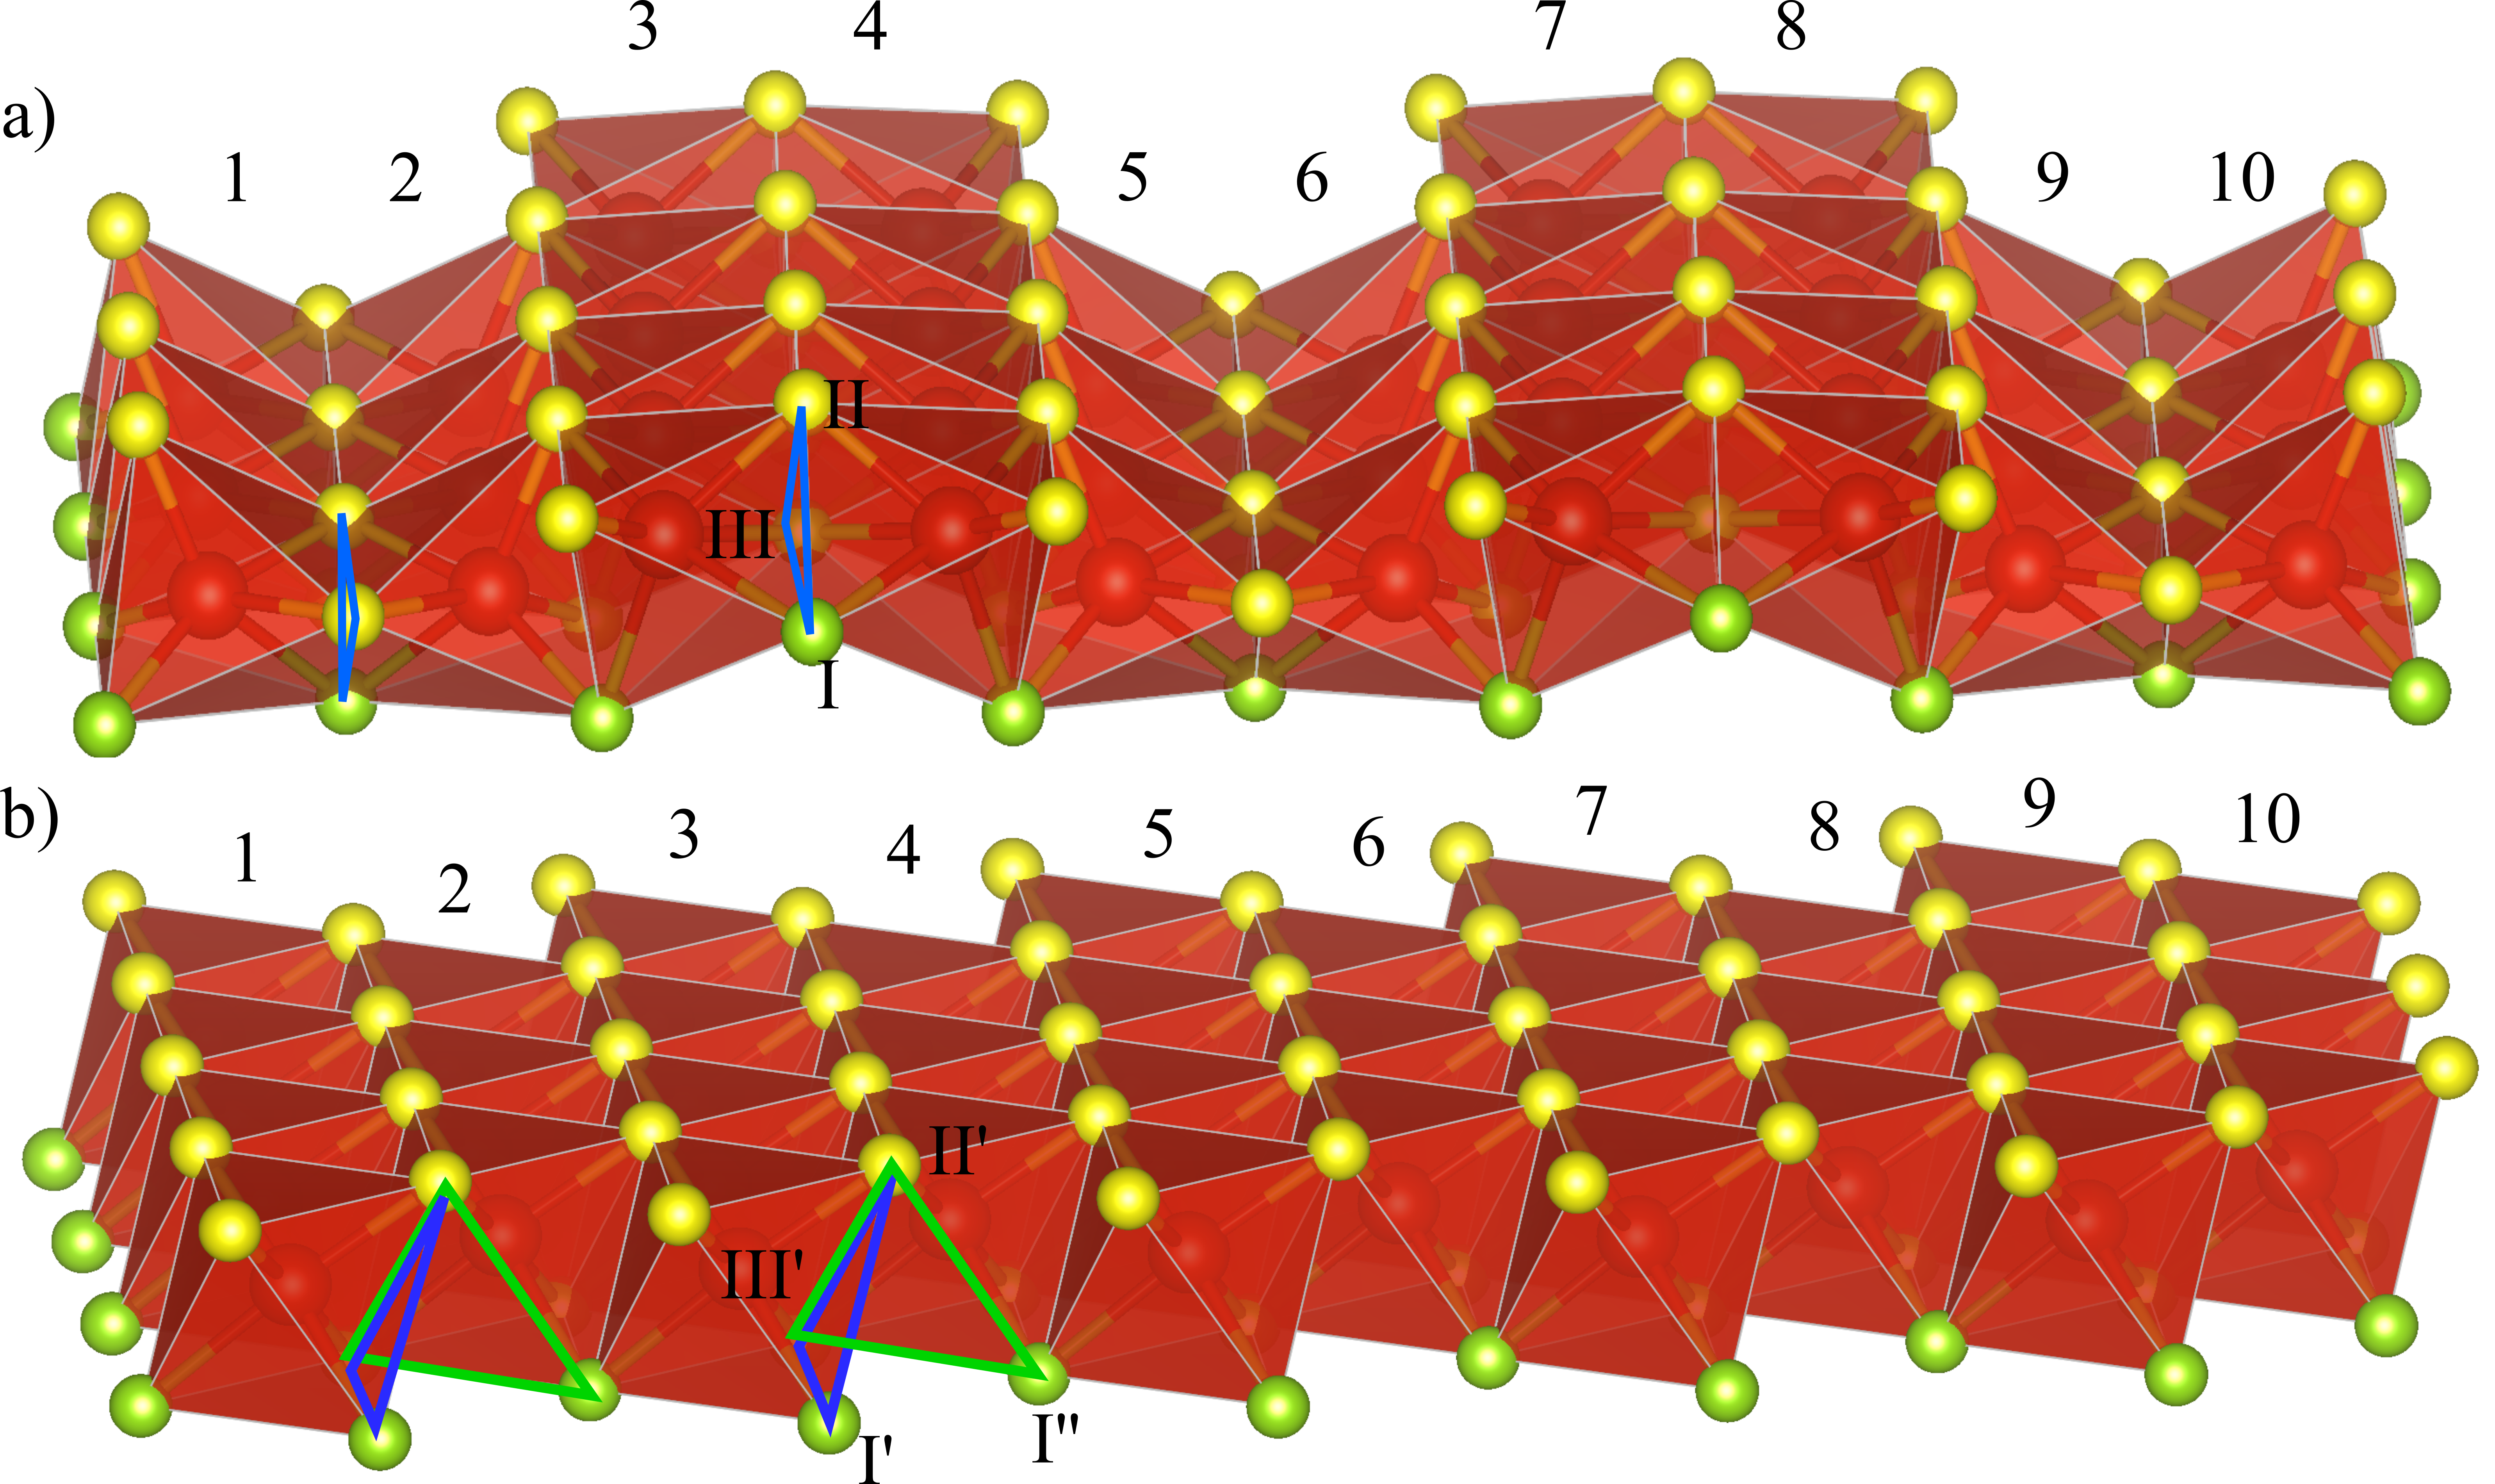
\includegraphics[width=0.8\textwidth]{T_hor_T.png} \\
	\caption{Comparison of 1M (a) and 1T (b) crystal structures; sulphur atoms are shown in yellow, selenium -- in green, vanadium -- in red colors, respectively.}
	\label{T_hor_T}
\end{figure}

\begin{figure}[H]
	\includegraphics[width=0.7\textwidth]{T_hor_slabs.png} \\
	\caption{The arrangement of double octahedral rows in 1M-SVSe (a) and 1T-SVSe (b) structures; the dashed lines show the common atoms in the adjacent slabs.}
	\label{T_hor_slabs}
\end{figure}


\begin{figure}[H]
	\includegraphics[width=0.4\textwidth]{T_hor_V.png} \\
	\caption{The comparison of the nets of V atoms in 1M-SVSe (a) and 1T-SVSe (b) crystal structures; the values of interatomic distances are given in \AA.}
	\label{T_hor_V}
\end{figure}

\begin{figure}[H]
        \includegraphics[width=0.5\textwidth]{T_hor_hcb.png} \\
        \caption{Top-view (a) and side-view (b) of the undulated nets of Ch atoms in 1M-SVSe structure.}
\label{T_hor_hcb}
\end{figure}



\paragraph{1M'-SMoSe}
Another structure with monoclinic symmetry sufficiently different from 1M phase was found using the USPEX package for SMoSe composition. 
This structure was called as SMoSe-1M'.
1M' is dynamically stable for SMoSe (Figure \ref{phon_smose}) and unstable for SVSe (Figure \ref{phon_svse}) chemical composition.

The enthalpy of 1M'-SMoSe is higher than the enthalpy of 1T-SMoSe on 0.05 eV/f.u. (Table \ref{t:str}). 

1M' structure is different from the other structures in that it is characterized by the almost right square net of Ch atoms (Figure \ref{H-hor}).
The bottom (selenium) layer is shifted relatively to top (sulfur) one (Figure \ref{H-hor}), while the transition metal atoms are arranged to have trigonal prismatic coordination.

Like in the 1H, in 1M' structure trigonal prisms share only common edges, but not common faces.
The difference between two structures is in that in 1H structure three-fold symmetry axis are perpendicular to the plane of monolayer, while in 1M' they are parallel to this plane.

Molybdenum atoms are connected by the bonds of 3.08--3.22 \AA\ lengths in quasi-1D chains (Figure \ref{H-hor_Mo}).
The chains are connected by the sufficiently weaker bonds of 4.08 \AA\ length (Figure \ref{H-hor_Mo}).


\begin{figure}[H]
	\includegraphics[width=\textwidth]{H-hor.png}
	\caption{The nets of sulfur (yellow) and selenium (green) atoms (a) and the arrangement of coordination polyhedra around Mo atoms (b) in 1M'-SMoSe.}
	\label{H-hor}
\end{figure} 


\begin{figure}[H]
	\includegraphics[width=0.4\textwidth]{H-hor_Mo.png}
	\caption{The chains of molybdenum atoms in 1M'-SMoSe.}
	\label{H-hor_Mo}
\end{figure} 


\paragraph{1A-SVSe and 1A'-SMoSe}
The structure with triclinic symmetry called 1A' was revealed with AIRSS package for SVSe composition.
Despite sufficient structural similarity between optimized 1A structure for SMoSe and SVSe compositions, there is an apparent crystallographic difference between them like that between 1T and 1T'.
Based on the fact mentioned, we will designate the structures as 1A-SVSe and 1A'-SMoSe.
Both 1A-SVSe and 1A'-SMoSe are dynamically stable (Figures \ref{phon_smose} and \ref{phon_svse}).

The enthalpy of 1A'-SVSe structure lies in-between the values of 1T and 1T' structures enthalpies, making 1A' more energetically favorable than 1T on nearly 0.1 eV/f.u.
For SMoSe composition, the ratio of enthalpies of the most favourable structures is the following: 
$H(1H) < H(1T') < H(1A) < H (1T)$.

In the case of SVSe composition, 1A phase is less favorable than 1T', 1T, and 1H structures (Table \ref{t:enthalpy}).

The 1A and 1A' structures can be better described based on the net of TM atoms, which forms the well-known kagome lattice \cite{zhang2021_kagome}, observed, for instance, in AV$_3$Sb$_5$ \cite{ortiz2021} and WO$_3$ \cite{gerand1979} compounds.
Kagome lattices of 1A-SVSe and 1A'-SMoSe structures, are not of ideal hexagonal symmetry, and there is the dispersion of bond lengths and deviation of bond angles from the ideal values of 120\textdegree.
In 1A'-SVSe, the bond lengths vary in the range of 3.07--3.49 \AA\ and bond angles –- in the rage of 115--122.9\textdegree\ (Figure \ref{airss1_tm}a).
In 1A'-SMoSe, the bond lengths are in the wide range of 2.78--3.79 \AA, and bond angles are in the range of 113.9--125.7\textdegree\ (Figure \ref{airss1_tm}b).
1A'-SMoSe is different from 1A-SVSe in that it is characterized by the presence of triangular clusters of TM atoms with sufficiently shorter bond lengths.
The bond lengths within clusters are equal to 2.78--2.81 \AA, while other Mo--Mo bonds are on 0.5--1 \AA\ longer (Figure \ref{airss1_tm}b).
In SMoSe-1T', the zig-zag chains of Mo atoms are connected by the bonds of 2.79 \AA\ length, i.e. they are equal to the bond lengths within triangular clusters.

1A and 1A' structures are characterised by the same nets of sulphur and selenium atoms (Figures \ref{airss1_s_comp} and \ref{airss3_S_Se}). 
The differences of bond angles and bonds lengths of sulphur nets of 1A-SVSe and 1A'-SMoSe structures do not exceed 0.1 \AA\ and 1\textdegree\ (Figure \ref{airss1_s_comp}).
The net of sulfur atoms is not planar, the deviation from the planar arrangement is nearly equal to $\pm$10\textdegree.
The sulfur net of 1A can be transformed into the sulfur net of 1H (or 1T) by the shift shown in Figure \ref{airss1_s} and subsequent deformations.


In 1A and 1A' structures, each TM atom is coordinated by Ch atoms arranged in highly deformed tetragonal pyramids.
The composition of such pyramids are (TM)S$_3$Se$_2$ or (TM)S$_2$Se$_3$.
The bond distances between TM and Ch atoms vary in the range of 2.26--2.58 \AA\ for 1A-SVSe and in the range of 2.29--2.63 \AA\ for 1A'-SMoSe. 
The pyramids are grouped in three, forming the triangles of TM atoms which correspond to the triangular rings of kagome lattice (Figure \ref{airss1_poly}).
There are the big holes between the triangular clusters of TM atoms, corresponding the hexagonal rings of kagome lattice (Figure \ref{airss1_poly}).



\begin{figure}
	\includegraphics [width=0.35\textwidth]{airss1_tm.png}
	\caption{The kagome atomic nets of TM atoms in 1A'-SVSe (a) and 1A-SMoSe (b) structures; triangular clusters of Mo atoms are highlighted in blue.} 
\label{airss1_tm}
\end{figure}

\begin{figure}
	\includegraphics[width=0.35\textwidth]{airss1v_s.png}
	\caption{The net of sulfur atoms in 1A-SVSe; dashed lines show the plane of the shift which transforms the net into the hexagonal net of 1T and 1H structures.}
\label{airss1_s}
\end{figure}


\begin{figure}[H]
        \includegraphics[width=0.35\textwidth]{airss1_v_poly.png}
        \caption{1A-SVSe with outlined coordination polyhedra around V atoms; the kagome lattice is outlined in black.}
\label{airss1_poly}
\end{figure}




\paragraph{1A''-SVSe and 1A'''-SMoSe}
One more crystal structure with triclinic symmetry was revealed for SVSe composition using AIRSS code and later was optimized for SMoSe composition.
Due to the apparent crystallographic difference of V- and Mo-based structures, they were designated as 1A''-SVSe and 1A'''-SMoSe.


Both considered structures are dynamically stable (Figures \ref{phon_smose} and \ref{phon_svse}).
The enthalpies of the 1A'' and 1A''' structures are higher than the enthalpies of 1H, 1T, and 1T' phases of the same chemical composition (Table \ref{t:enthalpy}).
1A''-SVSe is more energetically favourable than 1S and 1H' structures on nearly 0.4 eV/f.u., while 1A'''-SMoSe is less favourable on the same value of energy (Table \ref{t:enthalpy}).


The differences of 1A'' and 1A''' structures can be clearly seen in the side-view.
In 1A''-SVSe, TM atoms are nearly in the same plane as Ch atoms, while in 1A'''-SMoSe TM atoms are in-between the layers of Ch atoms.

The nets of chalcogen atoms of these phases are also sufficiently different.
In 1A''-SVSe, the topology of the net corresponds to the graphite-like hexagonal net (Figure \ref{airss3_svse}a), while in 1A'''-SMoSe chalcogen atoms form a triangular net if the weak contacts of 4.58-4.64 \AA\ are considered (Figure \ref{airss3_smose}a).
The new crystal-chemical feature of 1A''-SVSe which was not observed for the other TMDs structures is the presence of S--S and Se--Se dimers with the bond length of 2.09 \AA\ and 2.37 \AA, respectively (Figures \ref{airss3_svse}a and \ref{airss3_S_Se}).
These bond lengths correspond to that in the crystals structures of elemental sulfur and selenium.
Other S--S and Se--Se bonds of 1A''-SVSe are  sufficiently longer, varying in the range of 3.17--3.73 \AA\ (Figures \ref{airss3_svse}a and \ref{airss3_S_Se}).
In 1A'''-SMoSe there are no clusters of Ch atoms, S--S bonds vary in the range of 3.24-3.79 \AA\ with the weak contacts of 4.58--4.64 \AA\ (Figure \ref{airss3_svse}a).

The nets of TM atoms in 1A'' and 1A''' phases are also drastically different, as it is illustrated in the Figures \ref{airss3_svse}b and \ref{airss3_smose}b.
1A'''-SMoSe is characterized by the presence of Mo--Mo dimers with the bond lengths of 2.85 \AA, while other bonds vary in the range of 3.04--3.74 \AA\ (Figure \ref{airss3_smose}b).
There are no such short bonds in 1A''-SVSe, in which V--V bonds smoothly vary in the range of 3.32--3.79 \AA.

TM atoms in 1A''-SVSe are five- and six-coordinated by Ch atoms (Figure \ref{airss3_poly}a).
Coordination polyhedra are deformed tetragonal pyramids and trigonal prisms, respectively.
1A'''-SMoSe is characterised by the lower coordination numbers.
Vanadium atoms in it are four- and five-coordinated, and the coordination polyhedra are deformed tetrahedron and trigonal bipyramid, respectively (Figure \ref{airss3_poly}b).
1A''-SVSe is characterized by the infinite quadruple chains of coordination polyhedra (Figure \ref{airss3_poly}a) and 1A'''-SMoSe -- by the single chains (Figure \ref{airss3_poly}b).
In both structures, coordination polyhedra in the chains are connected through the common edges (Figure \ref{airss3_poly}).
The adjacent chains in 1A''-SVSe are connected through the common edges, while in 1A'''-SMoSe -- through the common vertices (Figure \ref{airss3_poly}).

\begin{figure}[H]
	\includegraphics[width=\textwidth]{airss3_side.png}
	\caption{The side-view of 1A''-SVSe (a) and 1A'''-SMoSe (b) structures.}
	\label{airss3_side}
\end{figure}

\begin{figure}[H]
	\includegraphics[width=0.5\textwidth]{airss3_svse.png}
	\caption{The nets of sulfur (a) and vanadium (b) atoms in 1A''-SVSe; vanadium atoms of the upper layer are highlighted.}
	\label{airss3_svse}
\end{figure}

\begin{figure}[H]
	\includegraphics[width=0.5\textwidth]{airss3_smose.png}
	\caption{The nets of sulfur (a) and molybdenum (b) atoms in 1A'''-SMoSe.}
	\label{airss3_smose}
\end{figure}


\begin{figure}[H]
	\includegraphics[width=\textwidth]{airss3_poly.png}
	\caption{Crystal structures of 1A''-SVSe (a) and 1A'''-SMoSe (b) with outlined coordination polyhedra.}
	\label{airss3_poly}
\end{figure}




%%%%%%%%%%%%%%%%%%%%%%%%%%%
\subsubsection{Analytically produced structures based on 1H}
%%%%%%%%%%%%%%%%%%%%%%%%%%

In this section, we considered crystal structures  which were produced analytically based on the 1H phase within the procedure which can  also be applied for the 1H' and 1S structures generation.
These structures, similarly to 1H' and 1S phases, can be considered as the possible structural models of grain boundaries.
As it will be shown below, the enthalpies of the obtained structures are not only higher than the enthalpies of 1H, 1T, and 1T' phases but also higher than enthalpies of 1H' and 1S.
However, we left their description here together with the description of 1H' and 1S phases to illustrate the formation of molybdenum dimers in SMoSe structures. 
Also, we would like to describe the procedure of the structures generation, which can be applied for the generation of other similar structures.

To construct new structures with TM atoms trigonal prismatic coordination we presented the structures as different fillings of the sulfur hexagonal nets of 1H structure (Figure \ref{H-based}).
1H TMDs phase presents the most symmetric chess-board-like filling (Figure \ref{H-based}a).
It should be noted that the 1S structure also have the chess-board-like filling, but with the doubled triangular cells having the rhombuses form (Figure \ref{H-based}b).
After the optimization these rhombuses transform into the the right squares (see Figure \ref{H-based}b).
There are two types of the empty rings in the 1H' structure: the first type is the primitive (non-centered) triangles, and the second one is the hexagon consisted of six triangular rings connected through the faces (Figure \ref{H-based}c).
The optimization does not sufficiently changes the forms of the empty rings, only slightly deforming the hexagons (Figure \ref{H-based}c).

Three new structures were produced in a similar way as it has been realised for 1H' and 1S phases. 
Two of them have orthorhombic symmetry and one -- the monoclinic one and we designated them as 1O, 1O', and 1M'' structures, respectively.
Structural data for SMoSe-1O, 1O', and 1M'' phases are given in {\it Supporting information} (Table \ref{t:str_test}).
Calculated phonon dispersion curves showed that in case of SMoSe composition 1O and 1M'' structures are dynamically stable (Figure \ref{phon_smose}), while in case of SVSe composition none of these structure is dynamically stable (Figure \ref{phon_smose}).
The enthalpies of 1O-SMoSe and 1M''-SMoSe are higher than the values of 1S-SMoSe and 1H'-SMoSe phases by approximately 0.1 eV/fu.

The analytical search was not able to propose new structures which follow the local charge balance principle, i.e. the structures in which each vertex of trigonal prism is common for three neighbouring prisms, as it is observed in 1H, 1H', and 1S phases. 
In the case of 1O phase, Ch atoms are common for two or four trigonal prisms, while in the cases of 1O' and 1M'' structures -- for two, three, or four trigonal prisms (Figure \ref{H-based}). 
It should be noted that 1M'' structure differs from the other structures: it is characterized by the presence of trigonal prisms having two common faces, while in all other structures the prisms share no more than one common face.
As it will be shown below, this fact is important for the formation of Mo--Mo dimers.
The optimisation of 1M'' structure sufficiently affects the arrangement of sulfur atoms: in the optimized 1M'' structure, the sulfur atoms net looses the hexagonal symmetry (Figure \ref{H-based}f), and Mo atoms are not only in trigonal prismatic but also in quadratic coordination (Figure \ref{H-based}f).


The presence of common edges and faces of [MoO$_6$] trigonal prisms in 1H', 1S, 1O, 1O', and 1M'' structures results in shorter Mo--Mo distances in comparison with 1H structure where the prisms have only common edges.
In 1H structure, Mo atoms form a regular hexagonal net in which all Mo--Mo bonds are equal to 3.25 \AA\ which corresponds to the edge-sharing disposition of trigonal prisms.

In 1H', 1S, and 1O structures Mo--Mo distances for edge-sharing disposition are equal to 2.9--3.8 \AA.
For face-sharing dispositions, the Mo--Mo distances is sufficiently shorter: in 1H' and 1S structures, they are equal to 2.9 \AA, in 1O -- to 2.75 \AA\ and in 1O' -- to 2.62 \AA.
As it was mentioned before, these values are close to Mo--Mo distances in the zig-zag chains of Mo atoms in the 1T' structure (2.75 \AA).
This value is in turn equal to the shortest distance between Mo atoms in the {\it bcc} structure of pure Mo (2.72 \AA) \cite{MoV}.
1M'' structure is characterized by the sufficiently shorter Mo--Mo bond, the distance between the adjacent Mo atoms in the dimer is equal to 2.22 \AA.
This short bond corresponds to quadruple Mo--Mo bond in Mo$_2^{4+}$ dimers, found in numerous organic molecules \cite{momo}.
Similar to organic molecules, in 1M'' structure  each molybdenum atom of Mo--Mo dimer is bound to four ligands that define almost right square (Figure \ref{test3_momo}).
Despite the relatively high enthalpy of the 1M'' structure its dynamic stability shows the theoretical possibility for the formation of quadruply bonded Mo$_2^{4+}$ dimers in metastable structures of TMDs and this was not considered before.

\begin{figure}[H] \centering
        \includegraphics[width=\textwidth]{H-based.png}
        \caption{SMoSe structures produced based on 1H. The numbers on polyhedra are represented to show the same fragment before and after the optimisation.}

\label{H-based}
\end{figure}

\begin{figure}[H]
	\includegraphics[width=0.3\textwidth]{test3_momo.png}
	\caption{A quadruple Mo--Mo bond in 1M''-SMoSe structure}
\label{test3_momo}
\end{figure}




%%%%%%%%%%%%%%%%%%%%%%%%
%\subsection{The uniqueness of the found structures}%может поменять на "Topological analysis"?
\subsection{The topological analysis}
%%%%%%%%%%%%%%%%%%%%%%%

To answer the question, whether the found structures are unique or if there are similar representatives in ICSD of CSD we performed the topological screening.
The obtained results showed that all found structures, except for 1M', are unique, and the similar structures were not found in the databases.
The same statement is true about the earlier known 1H' and 1S structures: similar structures for them were not also found. 
The 1M' structure belongs to the same {\bf kgd} topological type as the 1T structure and this means that 1M' can be transformed into the 1T phase without breaking the bonds.
However, the geometrical difference of 1M' and 1T structures is sufficient and the transformation of one structure into the other requires changing of the coordination polyhedron from the trigonal prism to the octahedron.

To evaluate the probability for synthesis of the 1A and 1A' structures on the substrate, we performed the search for the structures with kagome lattices of vanadium or molybdenum atoms.
As the result, 17 structures containing flat kagome lattice of vanadium atoms and no structures with the flat lattice of molybdenum atoms were found. 
The lengths of V--V bonds in the revealed structures vary in the range of 2.43--2.81 \AA.
This is close to the bonds lengths in the mentioned triangular clusters of Mo atoms and sufficiently higher than the lengths of V--V bonds in kagome net of 1A-SVSe phase.
Thus, based on the structures presented in ICSD it is problematic to suggest the proper substrate for the synthesis of 1A or 1A' structures.

It is worth noting, that mainly ICSD is the databse of experimentally syntheized 3D structures and  some structures synthesized in the form of monolayers or theoretically predicted ones can be not included in it.



\section{Discussion}

The discussion is devoted to possibility of practical applications of the found structures based on the correlation between structure features and physical properties. As all investigated structures consist of TM atoms surrounded by Ch atoms, the $d$-electrons levels of TM undergo splitting depending on the local symmetry. The crystal field theory proceeds from the fact that the nature of ligands and their location around the central ion (symmetry of the complex) reduce the degeneracy of $d$-orbitals and change their energy. Thereby the correlation between the structure and the electronic properties can be interpreted in terms of the crystal field theory.
According to the crystal field theory, in an octahedral environment (1T polymorph), the $d$-shell splits into a low-energy triplet (t2g) and a high-energy doublet (eg). In a trigonal prismatic geometry (1H), the low-energy triplet further splits into a doublet and a singlet \cite{pasquier2019crystal}. 
The two polymorphs of MoS$_2$ have distinct electronic properties, the 1H-MoS$_2$ phase is a semiconductor and the 1T-MoS$_2$ is metallic. The 1S-SMoSe despite the prismatic environment of TM atoms becomes a semi-metal \cite{lai2021catalytic, tang2021lattice} and Mo- and W-based 1H' structures are gapless semiconductors or, alternatively, semimetals \cite{ma2016two}. 
The proposed structure 1A' is characterized by a distorted trigonal bipyramidal local environment of the TM atom, which should make this structure more metallic due to degenerated $d$-orbitals. 
The square-pyramidal environment in 1A''' with the TM atom on the facet suggest the possibility for the application of this structure for molecular sorption and detection \cite{nano12050774}.
We believe that the proposed variety of phases of Janus TMDs in the future can significantly expand the scope of their application.

\section{Conclusions}
Using analytical analysis and computational algorithms within USPEX and AIRSS program packages we performed a theoretical prediction of novel Janus-type phases of TMDs with Mo-S and V-S compositions. We proposed some new phases of Janus TMDs called: 1M, 1M', 1M'', 1A, 1A', 1A'', 1A''', 1O and some of the structures proposed (1A'-SMoSe, 1A-SVSe, 1M-SVSe) not only demonstrate the stability according to the results of the phonon spectra calculation of but also have an enthaly similar to the already known phases (1H, 1T, 1T') of TMDs. We believe that with this work we are opening a discussion about the possible synthesis of new phases of Janus TMDs and further in-depth study of their properties.



\section*{Acknowledments}
The authors acknowledge financial support from Russian Science Foundation (№ 21-73-20183).

The authors are grateful to the Joint Supercomputer Center of the Russian Academy of Sciences and to the Information Technology Center of Novosibirsk State University for providing access to the cluster computational resources.

\bibliography{2d}
\bibliographystyle{CGD}


\end{document}


Comment. 
fes structure denoted as S-MS2 in \cite{tang2021_smose}.
fxt structure denoted as H' in \cite{ma2016_h'}.
Similarly there is T' – deformed T-phase.
We can follow this notation, designating our phases by symmetry with addition of '.


2.43--2.56 -- Ta2V3Si
2.81475		-- CaV3Sb4
2.74090		--KV3Sb5
2.53143		--CoVZr
2.61895		-- Vanadium \cite{vanadium}
2.72019		-- molybdenum \cite{molybdenum}

In H-hor structure, atoms of transition metal is in trigonal prismatic coordination, similarly to 1Н structure.
The difference between 1H and H-hor structures is in that in H-hor three-folld symmetry axis of trigonal prism is parallell to the plane of the layer, while in 1H it is perpendicular.

T-hor structure is characterized by the uniqe topology– 3,3,5,8-coordinated net if short V--V bonds are considered and 3,3,5,6-coordinated net if V--V bonds are not considered.
We have not found analogues of these nets in ICSD.

among which are Ta$_2$V$_3$Si \cite{Ta2V3Si}, CaV$_3$Sb$_4$ \cite{ CaV3Sb4}, KV$_3$Sb$_5$ \cite{KV3Sb5}, and CoVZr \cite{ZrVCO}.
The structures with kagome lattice of molybdenum have not been revealed.
The structures of pure vanadium or molybdenum are characterized by the similar bond lengths, which are equal to 2.62 \AA\ \cite{MoV} and 2.72 \AA\ \cite{MoV}, respectively.

Although 1H and 1T structures are characterized by the different coordination polyhedra, they are similar in the manner of polyhedra interconnection.
The 1H structure consists of trigonal prisms [MX$_6$], and 1T structure –- of the [MX$_6$] octahedra.
Each trigonal prism share all three vertical edges with the neighbouring prisms (Figure \ref{1H1T}a); each vertex of the trigonal prism is common for two other prisms (Figure \ref{1H1T}a).
Similarly in 1T structure, each octahedron share all inclined edges with neighbouring octahedra, and no common faces; each vertex is common for three octahedra (Figure \ref{1H1T}b).
Bond valence of M--X bond is  equal to +4/6 and there are necessary three such a bonds to compensate negative charge of S$^{2-}$ anion.
Thus, local charage balance are perfectly realized in both 1H and 1T.
As it will be shown below this is not the obligatory requirement and some of the found structures does not have the local charge balance.

Only interconnection of the coordination polyhedra through the common edges is realized in 1H and 1T structure.
Below, we will show examples of the structures, with face sharing of coordination polyhedra and enthalpy lower that of 1T structure of the same composition.

In contrast to trigonal prisms, the face-sharing of the octahedra seems to be problematic for quasi 2D structure because it results in the deviation from the flat arrangement.
However, as it will be shown below, the dynamically stable quasi-2D structure characterised by the face-sharing of octahedra was also predicted.
